\originalchapter{作业二：联合概率与变量变换}
\psource{8.044，2013 春，PS2，2 月 20 日截止。中文题面；据官方答案核对的 AI 独立解答。}
\originalsection{1．两个量子粒子}
\begin{exercise}
一维两粒子波函数 $\psi(x_1,x_2)=(\sqrt\pi x_0)^{-1}(x_2-x_1)x_0^{-1}\exp[-(x_1^2+x_2^2)/(2x_0^2)]$，$x_0>0$。(a) 求联合密度，在平面标明极大与极小；(b) 求各粒子的位置密度，判断独立性；(c) 求并画 $p(x_1\mid x_2)$。即使没有相互作用，量子态仍可产生这种相关性。
\end{exercise}
\begin{solution}
(a) $p=(x_2-x_1)^2e^{-(x_1^2+x_2^2)/x_0^2}/(\pi x_0^4)$；对角线 $x_1=x_2$ 为零，极大在 $(x_1,x_2)=(\mp x_0/\sqrt2,\pm x_0/\sqrt2)$。(b) 用高斯的零、一、二阶积分，
\[p_1(x)=p_2(x)=\frac{e^{-x^2/x_0^2}}{\sqrt\pi x_0}\left(\frac{x^2}{x_0^2}+\frac12\right).\]
联合密度不等于边缘乘积，故不独立。(c) $p(x_1\mid x_2)=e^{-x_1^2/x_0^2}(x_1-x_2)^2/[\sqrt\pi x_0(x_2^2+x_0^2/2)]$，在 $x_1=x_2$ 为零，两峰在 $x_1=(x_2\pm\sqrt{x_2^2+4x_0^2})/2$。下图给 $x_2=0$ 和 $x_2=x_0$ 两个代表截面。
\end{solution}
\begin{center}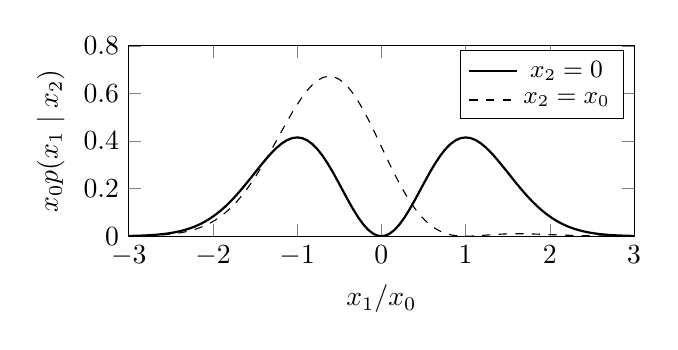
\begin{tikzpicture}\begin{axis}[width=8cm,height=4cm,xmin=-3,xmax=3,ymin=0,ymax=.8,xlabel={$x_1/x_0$},ylabel={$x_0p(x_1\mid x_2)$},samples=100,legend style={font=\small}]
\addplot[domain=-3:3,thick]{2*x*x*exp(-x*x)/sqrt(pi)};\addlegendentry{$x_2=0$}
\addplot[domain=-3:3,dashed]{(x-1)^2*exp(-x*x)/(1.5*sqrt(pi))};\addlegendentry{$x_2=x_0$}\end{axis}\end{tikzpicture}\end{center}
\begin{center}\begin{tikzpicture}[scale=1.1]\draw[->](-1.7,0)--(1.8,0)node[right]{$x_1/x_0$};\draw[->](0,-1.7)--(0,1.8)node[above]{$x_2/x_0$};\draw[dashed](-1.4,-1.4)--(1.4,1.4)node[right]{密度零};\fill(-.707,.707)circle(2pt)node[left]{极大};\fill(.707,-.707)circle(2pt)node[right]{极大};\end{tikzpicture}\end{center}
\originalsection{2．金字塔密度}
\begin{exercise}
在 $x\ge0,y\ge0,x+y\le1$ 上 $p(x,y)=6(1-x-y)$，其他处零。(a) 求并画 $p(x)$；(b) 求并画 $p(y\mid x)$。
\end{exercise}
\begin{solution}
积分得 $p(x)=3(1-x)^2$（$0\le x\le1$）。$p(y\mid x)=2(1-x-y)/(1-x)^2$（$0\le y\le1-x$，$0\le x<1$），为截距 $2/(1-x)$、底边 $1-x$ 的三角形；$x=1$ 为零概率条件，密度不能由此比值定义。
\end{solution}
\begin{center}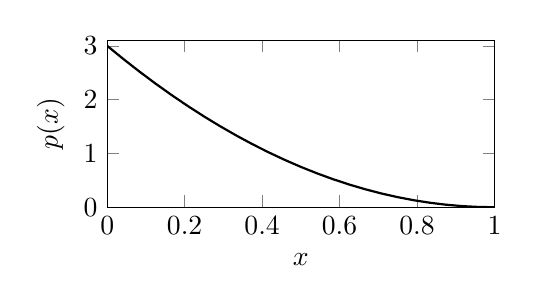
\begin{tikzpicture}\begin{axis}[width=6.5cm,height=3.7cm,xmin=0,xmax=1,ymin=0,ymax=3.1,xlabel={$x$},ylabel={$p(x)$}]\addplot[domain=0:1,thick]{3*(1-x)^2};\end{axis}\end{tikzpicture}\hspace{.3cm}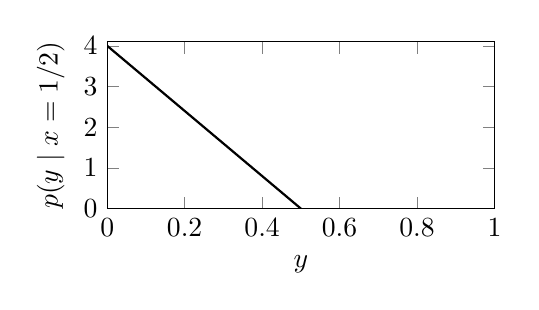
\begin{tikzpicture}\begin{axis}[width=6.5cm,height=3.7cm,xmin=0,xmax=1,ymin=0,ymax=4.1,xlabel={$y$},ylabel={$p(y\mid x=1/2)$}]\addplot[domain=0:.5,thick]{8*(.5-x)};\addplot[domain=.5:1]{0};\end{axis}\end{tikzpicture}\end{center}
\originalsection{3．最近邻恒星}
\begin{exercise}
恒星为空间泊松过程，平均密度 $\rho$（光年$^{-3}$）。(a) 求最近邻距离 $r$ 的密度；(b) 将总引力加速度 $\sum_i GM_i\vct r_i/|\vct r_i|^3$ 近似为最近邻质量 $M$ 产生的 $a=GM/r^2$，给出 $p(a)$ 与 $p(r)$ 的关系，指出忽略远邻在哪端误差最大；(c) 求均匀密度模型的 $p(a)$，近距离双星等会改变哪端；(d) 与观测比较还需考虑哪个随机量？
\end{exercise}
\begin{solution}
(a) $\Pr(r>R)=e^{-4\pi\rho R^3/3}$，所以 $p_r=4\pi\rho r^2e^{-4\pi\rho r^3/3}$。(b) $p_a(a)=p_r(\sqrt{GM/a})\sqrt{GM}/(2a^{3/2})$；小 $a$ 端最近邻较远，许多远邻不可忽略。(c)
\[p_a(a)=2\pi\rho(GM)^{3/2}a^{-5/2}\exp[-(4\pi\rho/3)(GM/a)^{3/2}],\quad a>0.\]
短距离结构影响大 $a$ 尾。原题称其 Holtsmark 分布；严格完整 Holtsmark 分布来自全部随机引力的向量和，上式只是最近邻近似。(d) 还需质量分布 $p(M)$，不能把所有星都当作同一个 $M$。
\end{solution}
\originalsection{4．理想气体动能}
\begin{exercise}
三维速度分量独立，$p(\vct v)=(2\pi\sigma^2)^{-3/2}e^{-v^2/(2\sigma^2)}$，$\sigma^2=\kb T/m$，$E=mv^2/2$。(a) 求能量密度，是否高斯；(b) 对表面吸附但平面内自由运动的二维气体做同样计算。
\end{exercise}
\begin{solution}
球壳或圆环测度给
\[p_{3D}(E)=\frac{2\sqrt E}{\sqrt\pi(\kb T)^{3/2}}e^{-E/(\kb T)},\qquad p_{2D}(E)=\frac1{\kb T}e^{-E/(\kb T)},\quad E\ge0.\]
二者均非高斯；第一种是形状 $3/2$ 的伽马分布，第二种是指数分布。
\end{solution}
\originalsection{5．由落点测速度}
\begin{exercise}
原子水平束沿正 $x$ 方向，靶距 $d$，重力下落 $s=A/v_x^2$，$A=gd^2/2$。测得
\[p_s(\zeta)=\frac{A^{3/2}}{\sigma^2\sqrt{2\pi\sigma^2}\,\zeta^{5/2}}\exp[-A/(2\sigma^2\zeta)],\quad\zeta>0.\]
负落距处为零。求并画源端速度密度。
\end{exercise}
\begin{solution}
只取 $v_x>0$，$|\dd s/\dd v_x|=2A/v_x^3$，故 $p_{v_x}(v)=2v^2e^{-v^2/(2\sigma^2)}/[\sigma^2\sqrt{2\pi\sigma^2}]$。从零升至 $v=\sqrt2\sigma$ 的峰，再指数下降；恰为正轴 Maxwell 速率形状，积分一。
\end{solution}
\begin{center}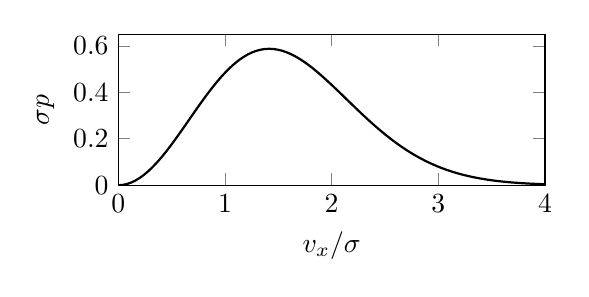
\begin{tikzpicture}\begin{axis}[width=7cm,height=3.5cm,xmin=0,xmax=4,ymin=0,ymax=.65,xlabel={$v_x/\sigma$},ylabel={$\sigma p$},samples=100]\addplot[domain=0:4,thick]{sqrt(2/pi)*x*x*exp(-x*x/2)};\end{axis}\end{tikzpicture}\end{center}
\originalsection{6．球壳为何成为亮环}
\begin{exercise}
低质量恒星抛出的发光球壳常呈亮环。设原子均匀分布在半径 $R$ 的球面，视线过球心，$r_\perp=R\sin\theta$。求原子到视线的垂距密度；可先求累计函数对应的两个球冠。官方题页的 Abell 39、Shapley 1 APOD 照片仅作现象示意，版权对象未转载，不影响题目。
\end{exercise}
\begin{solution}
$\cos\theta$ 在 $[-1,1]$ 均匀，$F(r)=1-\sqrt{1-r^2/R^2}$（$0\le r\le R$），所以 $p(r)=r/[R^2\sqrt{1-r^2/R^2}]$。每单位投影面积的密度 $p(r)/(2\pi r)$ 在边缘可积发散，形成临边增亮。有限壳厚与分辨率会抹平发散。
\end{solution}
